\capitulo{1}{Introducción}

\section{Descripción}

Los Sistemas de Gestión del Aprendizaje (LMS), como Moodle, se han consolidado como plataformas fundamentales en el ámbito educativo. A pesar de la gran cantidad de datos que generan sobre la actividad del alumnado, Moodle no dispone por defecto de herramientas visuales orientadas al profesorado que faciliten un análisis del aprendizaje \cite{learning-analytics} de forma ágil e intuitiva. Para dar una respuesta eficaz a esta necesidad surgió UBUMonitor, una robusta aplicación de escritorio de código abierto \cite{ubumonitor} que se ha convertido en una herramienta de gran valor y referente para que los docentes monitoricen la actividad, calificaciones y finalización de tareas de sus estudiantes. Esta excelente plataforma, destaca por una arquitectura ingeniosa que descarga los datos mediante servicios web y los almacena en una caché local cifrada (Blowfish), garantizando un trabajo sin conexión fluido y protegiendo de forma estricta la privacidad de los datos. Además, su continua evolución ha permitido incorporar algoritmos de aprendizaje no supervisado (clustering) muy avanzados para el descubrimiento de perfiles y patrones de comportamiento en el alumnado.

Tomando como sólida base el diseño funcional y la madurez tecnológica de la herramienta original, este Trabajo Fin de Grado (TFG) presenta UBUMonitorWeb. El objetivo principal de este proyecto es expandir el alcance de UBUMonitor mediante una evolución arquitectónica que traslade sus capacidades a un entorno de naturaleza web, operando bajo un modelo cliente-servidor. Compuesto por un servicio backend desarrollado con Spring Boot (utilizando Kotlin DSL) y un cliente frontend en Angular, el sistema funciona de manera integrada y se distribuye como una aplicación indivisible.

\begin{figure}
    \centering
    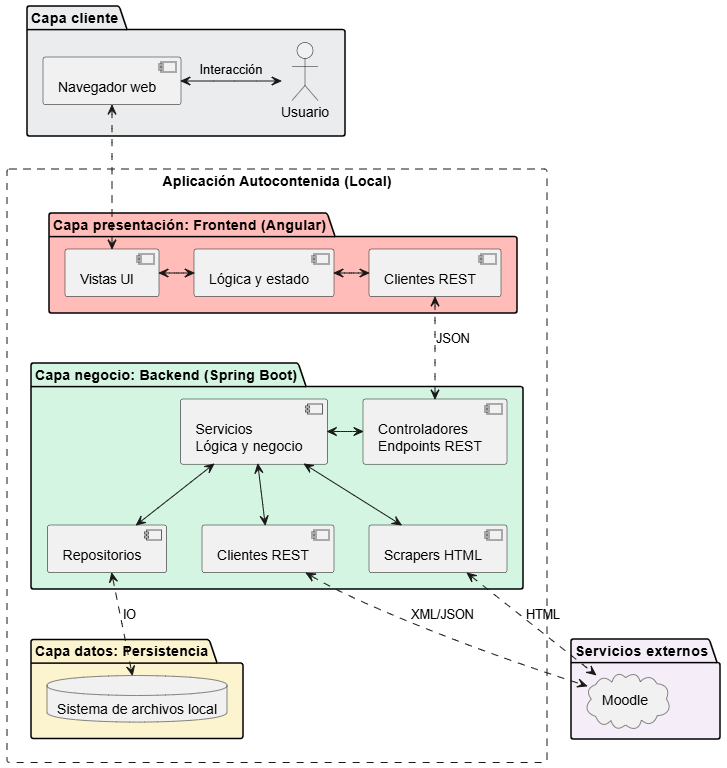
\includegraphics[width=01\linewidth]{img/diagram1-architecture.png}
    \caption{Diagrama de arquitectura}
    \label{fig:placeholder}
\end{figure}

Este desarrollo busca complementar a la versión de escritorio, abriendo nuevas vías de despliegue tecnológico y aportando las siguientes características:

\begin{itemize}
    \item \textbf{Versatilidad en el despliegue:} Heredando la filosofía de facilidad de uso, la aplicación se distribuye como un único fichero en dos modalidades. Por un lado, un ejecutable Java WAR tradicional, dependiente de Java Runtime Environment (JRE) 25. Y, por otro lado, como ejecutables nativos compilados con GraalVM \cite{graalvm} para Windows, GNU/Linux y MacOS; estos incluyen todo lo necesario para ejecutarse de forma totalmente independiente, ofreciendo tiempos de arranque muy reducidos y un consumo de memoria altamente eficiente.

    \item \textbf{Arquitectura embebida y visualización web:} La aplicación se despliega sobre un servidor Tomcat embebido que expone un servicio web (API REST) disponible por defecto en \url{http://localhost:8080}. Al acceder a esta ruta, se sirve la aplicación PWA Angular previamente compilada como contenido estático. Para la representación gráfica en el navegador, se ha integrado la librería Apache ECharts, la cual aprovecha el ecosistema web para ofrecer visualizaciones interactivas que enriquecen y complementan el excelente conjunto de gráficas ya ideado en la versión de escritorio.

    \item \textbf{Comunicación con Moodle y eficiencia de datos:} Se mantienen los estándares de integración de la herramienta original, soportando autenticación mediante credenciales tradicionales y Single Sign-On (SSO). La comunicación (HTTP/S) utiliza técnicas híbridas de \textit{web scraping} y servicios web nativos de Moodle. Los datos se solicitan una única vez tras el inicio de sesión y la selección del curso, reduciendo el tráfico de red. Los datos se mantienen en memoria para garantizar una fluidez total y el usuario puede exportarlos a un fichero cifrado local, lo que permite ``rehidratar'' sesiones posteriores de forma instantánea.

    \item \textbf{Módulo de análisis de texto no estructurado:} Como nueva aportación al ecosistema de la herramienta, se ha implementado un módulo inspirado en Grok (ElasticSearch). Definiendo patrones de inferencia, permite transformar registros crudos de Moodle en datos estructurados a través de plantillas flexibles. Esta funcionalidad, basada en registros reales o previamente anonimizados, brinda una nueva capa de extensibilidad.
\end{itemize}

\section{Estructura de la memoria}

Para detallar el proceso de diseño e implementación de UBUMonitorWeb, este documento se ha estructurado en los siguientes capítulos:

\begin{itemize}
    \item Capítulo 1: Introducción. Expone el contexto, la descripción general de la herramienta desarrollada y la estructura del documento.

    \item (TODO)
\end{itemize}


Materiales entregados:
\begin{itemize}
    \item \textbf{Tablero de gestión de proyecto (\textit{Kanban}):} Trablero integrado mediante la herramiento GitHub Projects, utilizado para la planificación ágil, el seguimiento del estado de las tareas (organizadas en columnas como Backlog, Todo, In-Progress, Done, Discarded) y la gestión general del ciclo de vida del desarrollo.\\
    \url{https://github.com/users/verteramo/projects/5/views/1?layout=board}
    
    \item \textbf{Código fuente:} Repositorio completo del proyecto alojado en GitHub, que incluye tanto el backend Spring Boot (\href{https://github.com/verteramo/UBUMonitorWeb/tree/main/api}{\texttt{/api}}) como el frontend Angular (\href{https://github.com/verteramo/UBUMonitorWeb/tree/main/app}{\texttt{/app}}).\\
    \url{https://github.com/verteramo/UBUMonitorWeb}

    \item \textbf{Releases:} Ejecutables precompilados en formato WAR y binarios nativos (compilados con GraalVM) para sistemas operativos Windows, GNU/Linux y MacOS.\\
    \url{https://github.com/verteramo/UBUMonitorWeb/releases}

    \item (TODO) 'Manual de usuario', 'Manual del programador', \dots
\end{itemize}